\documentclass[11pt]{amsbook}

\usepackage{../Ceyhun}	% ------------------------


\begin{document}

% ++++++++++++++++++++++++++++++++++++++
\hPage{ceyhun/069}
% ++++++++++++++++++++++++++++++++++++++

% =======================================
   
   oluşturduğu \underline{oluşuk çizge} \(C_1[C_2]\)
   \\a) \(d_1_i\), \(d_1_k\)ye bitişikse ya da
   \\b) \(d_1_i = d_1_k\) ve \(d_2_j\), \(d_2_l\)ye bitişikse koşullardan biri sağlandığında, (\(d_1_i\), \(d_2_i\)) ve (\(d_1_k\), \(d_2_l\)) düğümleri arasında bir ayrıtı bulunan çizge olarak tanımlanır.

% =======================================
   \\ Şekil 2.3.4 te \(C_1[C_2]\) ve \(C_2[C_1]\) oluşuk çizgeleri gösterilmiştir.
   \[ C_1 + C_2 = C_2 + C_1\]
   ve
   \begin{center}
   \\\(C_1\) x \(C_2\) = \(C_2\) x \(C_1\)
    \end{center}
    eşitliklerine karşın, genellikle, 
    \[ C_1[C_2] \neq C_2[C_1]\]
    olacaktır(Hangi koşullar altında bu eşitsizliğin eşitliğe dönüşeceğini inceleyiniz).
     \\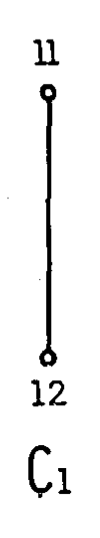
\includegraphics[scale = 0.7]{images/ceyhun-069_fig1}
    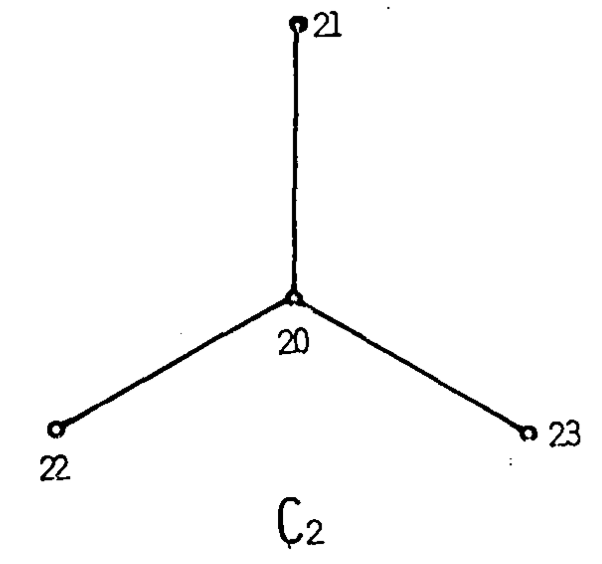
\includegraphics[scale = 0.7]{images/ceyhun-069_fig2}
% =======================================================
  
% =======================================

\end{document}  

%==== templates ====

%==== environments ====

%\begin{figure}[htb]
%	\centering
%	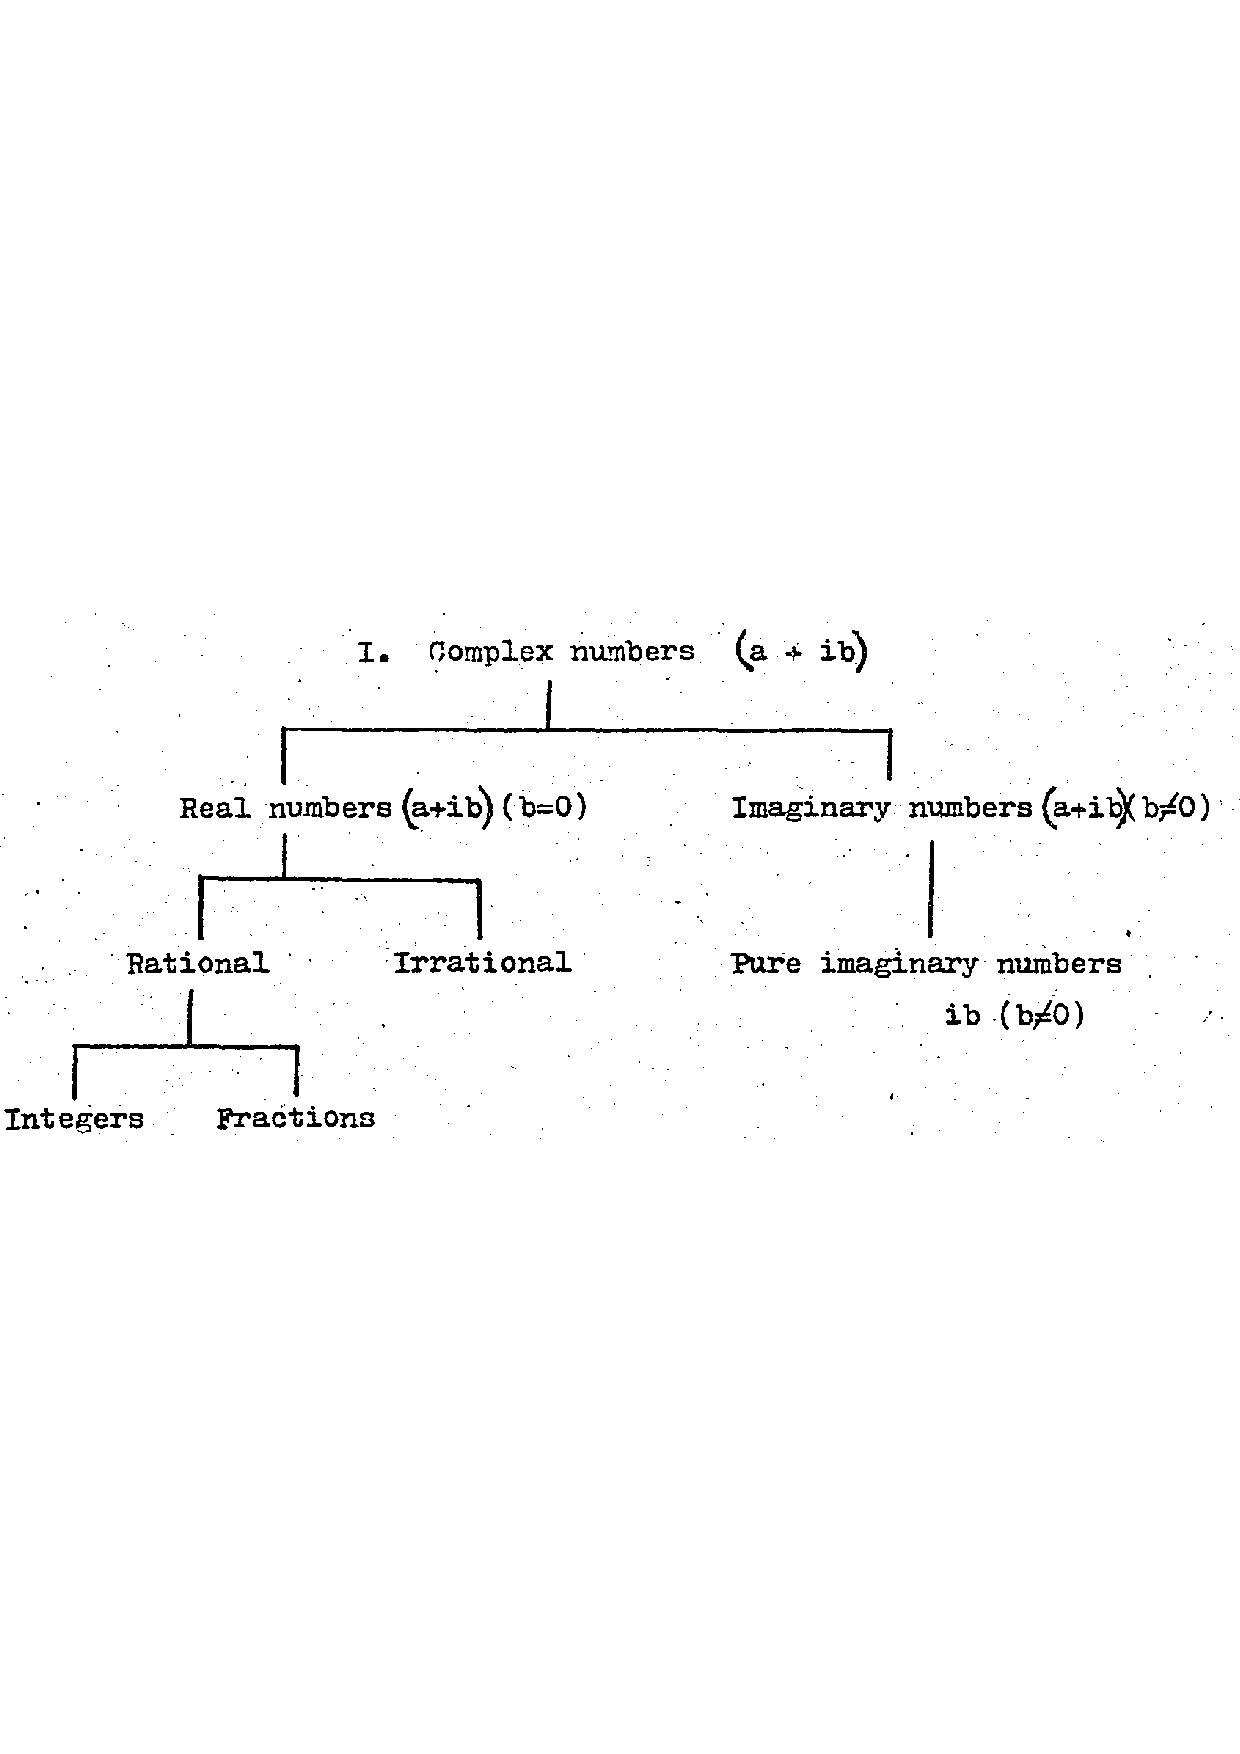
\includegraphics[width=0.9\textwidth]{images/SD-1-1p15A}
%	\caption{Classification of complex numbers}
%	\label{fig:classificationOfComplexNumbersA}
%\end{figure}

%\begin{center}
%\begin{tabular}{cc}
%\end{tabular}
%\end{center}

%\begin{exmp}
%\begin{hSolution}
%\end{hSolution}
%\end{exmp}

%\begin{hEnumerateAlpha}
%\end{hEnumerateAlpha}

%\begin{hEnumerateRoman}
%\end{hEnumerateRoman}

%$
%\begin{bmatrix}
%\end{bmatrix}
%$

%\frac{aaaa}{bbb}
%\frac{a_{n}}{b_{n}}
%\left( aaaa \right)
%\Longrightarrow

%\begin{multicols}{2}
%	bb
%\columnbreak
%	aa
%\end{multicols}